\documentclass{standalone}

\usepackage{tikz}

\begin{document}
  %noformat{
  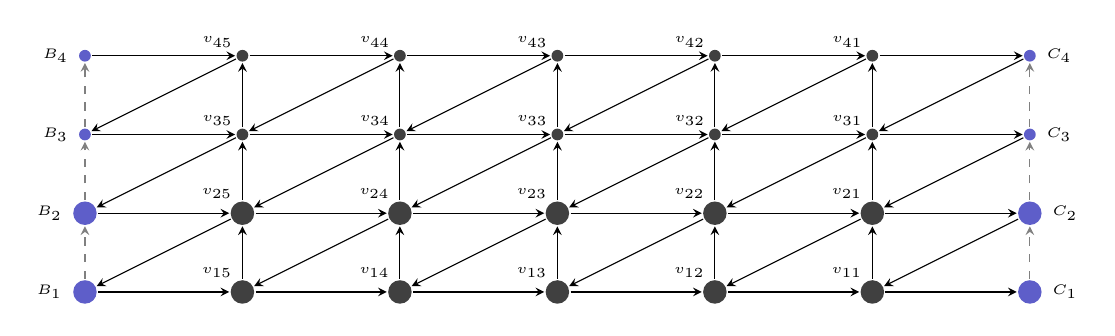
\begin{tikzpicture}
    \tikzstyle{v1} = [circle, outer sep=0.5pt, fill, inner sep=1.5pt]
    \tikzstyle{v2} = [circle, outer sep=0.5pt, fill, inner sep=3.0pt]
    \tikzstyle{unf} = [color=darkgray]
    \tikzstyle{frz} = [color=blue!60!darkgray!70]
    \tikzstyle{e} = [->, >={stealth}]
    \tikzstyle{h} = [dashed, color=gray, ->, >={stealth}]

    \tikzset{font=\tiny}

    \node[v2,label={0:{$C_1$}}, frz] (v10) at (12,0) {};
    \node[v2,label={0:{$C_2$}}, frz] (v20) at (12,1) {};
    \node[v1,label={0:{$C_3$}}, frz] (v30) at (12,2) {};
    \node[v1,label={0:{$C_4$}}, frz] (v40) at (12,3) {};

    \node[v2,label={[label distance=-3pt]95:{$v_{11}$}}, unf] (v11) at (10,0) {};
    \node[v2,label={[label distance=-3pt]95:{$v_{21}$}}, unf] (v21) at (10,1) {};
    \node[v1,label={[label distance=-3pt]95:{$v_{31}$}}, unf] (v31) at (10,2) {};
    \node[v1,label={[label distance=-3pt]95:{$v_{41}$}}, unf] (v41) at (10,3) {};

    \node[v2,label={[label distance=-3pt]95:{$v_{12}$}}, unf] (v12) at (8,0) {};
    \node[v2,label={[label distance=-3pt]95:{$v_{22}$}}, unf] (v22) at (8,1) {};
    \node[v1,label={[label distance=-3pt]95:{$v_{32}$}}, unf] (v32) at (8,2) {};
    \node[v1,label={[label distance=-3pt]95:{$v_{42}$}}, unf] (v42) at (8,3) {};

    \node[v2,label={[label distance=-3pt]95:{$v_{13}$}}, unf] (v13) at (6,0) {};
    \node[v2,label={[label distance=-3pt]95:{$v_{23}$}}, unf] (v23) at (6,1) {};
    \node[v1,label={[label distance=-3pt]95:{$v_{33}$}}, unf] (v33) at (6,2) {};
    \node[v1,label={[label distance=-3pt]95:{$v_{43}$}}, unf] (v43) at (6,3) {};

    \node[v2,label={[label distance=-3pt]95:{$v_{14}$}}, unf] (v14) at (4,0) {};
    \node[v2,label={[label distance=-3pt]95:{$v_{24}$}}, unf] (v24) at (4,1) {};
    \node[v1,label={[label distance=-3pt]95:{$v_{34}$}}, unf] (v34) at (4,2) {};
    \node[v1,label={[label distance=-3pt]95:{$v_{44}$}}, unf] (v44) at (4,3) {};

    \node[v2,label={[label distance=-3pt]95:{$v_{15}$}}, unf] (v15) at (2,0) {};
    \node[v2,label={[label distance=-3pt]95:{$v_{25}$}}, unf] (v25) at (2,1) {};
    \node[v1,label={[label distance=-3pt]95:{$v_{35}$}}, unf] (v35) at (2,2) {};
    \node[v1,label={[label distance=-3pt]95:{$v_{45}$}}, unf] (v45) at (2,3) {};

    \node[v2,label={180:{$B_{1}$}}, frz] (v16) at (0,0) {};
    \node[v2,label={180:{$B_{2}$}}, frz] (v26) at (0,1) {};
    \node[v1,label={180:{$B_{3}$}}, frz] (v36) at (0,2) {};
    \node[v1,label={180:{$B_{4}$}}, frz] (v46) at (0,3) {};

    \foreach \p in {0, 6} {
      \draw[h] (v1\p) -- (v2\p);
      \draw[h] (v2\p) -- (v3\p);
      \draw[h] (v3\p) -- (v4\p);
    }
    \foreach \p in {1, 2, 3, 4, 5} {
      \draw[e] (v1\p) -- (v2\p);
      \draw[e] (v2\p) -- (v3\p);
      \draw[e] (v3\p) -- (v4\p);
    }
    \foreach \p/\q in {0/1, 1/2, 2/3, 3/4, 4/5, 5/6} {
      \draw[e] (v1\q) -- (v1\p);
      \draw[e] (v2\q) -- (v2\p);
      \draw[e] (v3\q) -- (v3\p);
      \draw[e] (v4\q) -- (v4\p);

      \draw[e] (v2\p) -- (v1\q);
      \draw[e] (v3\p) -- (v2\q);
      \draw[e] (v4\p) -- (v3\q);
    }

  \end{tikzpicture}
  %}noformat
\end{document}
